% !TEX root = ../main.tex
%
% ========
\chapter{Particle interferometry}
% ========
  Two-particle interferometry (also called \textit{femtoscopy}) gives a possibility to investigate space-time characteristics of the particle-emitting source created in heavy ion collisions.
  Through the study of particle correlations, their momentum distributions can be used to obtain information about the spatial extent of the created system.
  Using this method, one can measure sizes of the order of $10^{-15}$ m and time of the order of $10^{-23}$ s.
  %
  % ========
  \section{HBT interferometry}
  % ========
    In the 1956 Robert Hanbury Brown and Richard Q. Twiss proposed a method which through analysis of interference between photons allowed to investigate angular dimensions of stars.
    The most important result from the Hanbury-Brown-Twiss experiments is that two indistinguishable particles can produce an interference effect.
    There is almost no difference between normal interferometry and HBT method, except that the latter one does not take into account information about phase shift of registered particles.
    At the beginning this method was used in astronomy for photon interference, but this effect can be used also to measure extent of any emitting source.
    This method was adapted to heavy ion collisions to investigate dimensions of a system created in those collisions by studying correlations of identical particles~\cite{nonidfemto}.
    The main difference between HBT method in astronomy and femtoscopy is that the first one is based on space-time HBT correlations and the latter one uses momentum correlations.
    The momentum correlations yield the space-time picture of the source, whereas the space-time HBT correlations provide the characteristic relative momenta of emitted photons, which gives the angular size of the star without the knowledge of its radius and lifetime~\cite{florkowski}.
  % \section{Intensity interferometry in heavy ion collisions}
  %
  % ========
  \section{Theoretical approach}
  % ========
    Intensity interferometry in heavy ion physics uses similar mathematical formalism as the astronomy HBT measurement.
    Through the measurement of correlation between particles as a function of their relative momentum one can deduce the average separation between emitting sources.

    %
    % ========
    \subsection{Conventions used}
    % ========
      In heavy ion collisions to describe particular directions, components of momentum and location of particles, one uses naming convention called the Bertsch-Pratt coordinate system.
      This system is presented in the Fig.~\ref{fig:coordinate-system}.
      \begin{figure}[h]
        \centering
        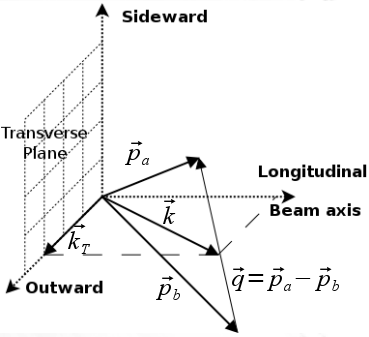
\includegraphics[width=0.5\textwidth]{coordinate_system}
        \caption{Bertsch-Pratt direction naming convention used in heavy ion collision.}
        \label{fig:coordinate-system}
      \end{figure}
      The three directions are called \textit{longitudinal}, \textit{outward} and \textit{sideward}.
      The longitudinal direction is parallel to the beam axis.
      The plane perpendicular to the beam axis is called a \textit{transverse plane}.
      A projection of a particle pair momentum $\vect{k} = (\vect{p}_a + \vect{p}_b)/2$ on a transverse plane (a \textit{transverse momentum} $\vect{k}_T$) determines \textit{outward} direction: $(\vect{k})_{out} = \vect{k}_T$.
      A direction perpendicular to the longitudinal and outward is called \textit{sideward}.

      A particle pair is usually described using two coordinate systems.
      The first one, \textit{Longitudinally Co-Moving System} (\textbf{LCMS}) is moving along the particle pair with the longitudinal direction, in other words, the pair longitudinal momentum vanishes: $(\vect{p}_a)_{long} = -(\vect{p}_b)_{long} $.
      The second system is called \textit{Pair Rest Frame} (\textbf{PRF}).
      In the PRF the centre of mass rests: $\vect{p}_a = -\vect{p}_b$.
      Variables which are expressed in the PRF are marked with a star (e.g. $\vect{k}^{*}$).

      The transition of space-time coordinates from LCMS to PRF is simply a boost along the outward direction, with the transverse velocity of the pair~$\beta_t = (\vect{v}/c)_{out}$~\cite{nonidfemto}:
      \begin{align}
        \label{eq:lcmstoprf}
        r^{*}_{out} &= \gamma_{t}(r_{out} - \beta_{t} \Delta t)\\
        r^{*}_{side} &= r_{side}\\
        r^{*}_{long} &= r_{long}\\
        \Delta t^{*} &= \gamma_{t}(\Delta t - \beta_{t} r_{out})~,
      \end{align}
      where $\gamma_{t} = (1-\beta^{2}_{t})^{-1/2}$ is the Lorentz factor.
      However, in calculations performed in this work the equal time approximation, which assumes that particles in a pair were produced at the same time in PRF - the $\Delta t^{*}$ is neglected.

      The most important variables used to describe particle pair are their total momentum $\vect{P} = \vect{p}_a + \vect{p}_b$ and relative momentum $\vect{q} = \vect{p_a} - \vect{p_b}$.
      In the PRF one has $\vect{q} = 2 \vect{k}^{*}$, where $\vect{k}^{*}$ is a momentum of the first particle in PRF.

    %
    % ========
    \subsection{Two particle wave function}
    % ========
      Let us consider two identical particles with momenta $\vect{p_1}$ and $\vect{p_2}$ emitted from space points $\vect{x_1}$ and $\vect{x_2}$.
      Those emitted particles can be treated as two incoherent waves.
      \begin{figure}[h]
        \centering
        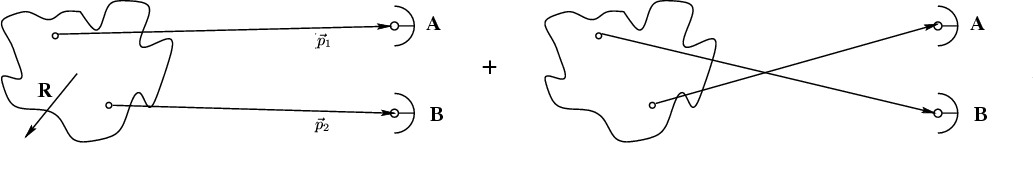
\includegraphics[width=0.9\textwidth]{wavefunction}
        \caption{The pair wave function is a superposition of all possible states. In case of particle interferometry it includes two cases: particles with momenta $p_1$,~$p_2$ registered by detectors \textit{A}, \textit{B} and $p_1$,~$p_2$ registered by \textit{B}, \textit{A} respectively.}
        \label{fig:wavefunction}
      \end{figure}
      If the particles are identical, they are also indistinguishable, therefore one has also take into account the scenario, where the particle with momentum $\vect{p_1}$ is emitted from $\vect{x_2}$ and particle $\vect{p_2}$ from $\vect{x_1}$ (Fig.~\ref{fig:wavefunction}).
      In such case, the wave function describing behaviour of a pair has to contain both components~\cite{drkisiel}:
      \begin{equation}
      \label{eq:wavefunction}
        \Psi_{ab}(\vect{q})=\frac{1}{\sqrt{2}} \left[ \exp(- i \vect{p_1}\vect{x_1} - i \vect{p_2}\vect{x_2}) \pm \exp(- i \vect{p_2}\vect{x_1} - i \vect{p_1}\vect{x_2}) \right]~.
      \end{equation}
      A two particle wave function of identical bosons is symmetric (``+'' sign in Eq.~\ref{eq:wavefunction}) and in case of identical fermions - antisymmetric (``-'' sign).
      This anti-symmetrization or symmetrization implies the correlation effect coming from the Fermi-Dirac or Bose-Einstein statistics accordingly.

      To provide full description of a system consisting of two charged hadrons, one has to include in the wave function besides quantum statistics also Coulomb and strong Final State Interactions.
      Considering identical particles systems, the quantum statistics is a main source of a correlation.
      Hence, in case of space-time analysis of particle emitting source, effects coming from the Coulomb and Strong interactions can be neglected.
    %
    % ========
    \subsection{Source emission function}
    % ========
      To describe particle emitting source, one uses a single emission function~\cite{nonidfemto}:
      \begin{equation}
        \label{eq:source-single-3d}
        S_A(\vect{x}_1,\vect{p}_1) = \int S(\vect{x}_1,\vect{p}_1,\vect{x}_2,\vect{p}_2,...,\vect{x}_N,\vect{p}_N)
        d \vect{x}_2 d \vect{p}_2 ... d \vect{x}_N d \vect{p}_N
      \end{equation}
      and a two-particle one:
      \begin{equation}
        \label{eq:source-two-3d}
        S_{AB}(\vect{x}_1,\vect{p}_1,\vect{x}_2,\vect{p}_2) = \int S(\vect{x}_1,\vect{p}_1,\vect{x}_2,\vect{p}_2,...,\vect{x}_N,\vect{p}_N)
        d \vect{x}_3 d \vect{p}_3 ... d \vect{x}_N d \vect{p}_N~.
      \end{equation}
      Emission functions $S(\cdot)$ can be interpreted as a probability to emit a particle, or a pair of particles from a given space-time point with a given momentum.
      In principle, the source emission function should encode all physics aspects of the particle emission process i.e. the symmetrization for bosons and fermions, as well as the two-body and many body Final State Interactions.
      Instead of this, one assume that each particle's emission process is independent - the interaction between final-state particles after their creation is independent from their emission process.
      The assumption of this independence allows to construct two-particle emission function from single particle emission functions via a convolution~\cite{nonidfemto}:
      \begin{equation}
        \label{eq:source-two-conv}
        \begin{split}
          S(\vect{k}^{*},\vect{r}^{*}) = \int S_A ( \vect{p}_1, \vect{x}_1 ) S_B ( \vect{p}_2, \vect{x}_2 )
          \delta \left[\vect{k}^{*} - \frac{\vect{p}_1+\vect{p}_2}{2} \right]
          \delta \left[\vect{r}^{*} - (\vect{x}_1+\vect{x}_2) \right] \\
          \times~d^4 \vect{x}_1 d^4 \vect{x}_2 d^4 \vect{x}_1 d^3 \vect{p}_1 d^3 \vect{p}_2
        \end{split}
      \end{equation}
      In case of identical particles, ($S_A = S_B$) several simplifications can be made.
      A convolution of the two same Gaussian distributions is also a Gaussian distribution with $\sigma$ multiplied by $\sqrt{2}$.
      Femtoscopy can give information only about two-particle emission function, but when considering Gaussian distribution as a source function in Eq.~\ref{eq:source-two-conv}, one can obtain a $\sigma$ of a single emission function from a two-particle emission function.
      The Eq.~\ref{eq:source-two-conv} is not reversible - an information about $S_A(\cdot)$ cannot be derived from $S_{AB}(\cdot)$.
      An exception from this rule is a Gaussian source function, hence it is often used in femtoscopic calculations.
      Considering pairs of identical particles, an emission function is assumed to be described by the following equation in the Pair Rest Frame~\cite{nonidfemto}:
      \begin{equation}
        S^{PRF}_{1D} (\vect{r}^{*}) = \exp \left( - \frac{ {r_{out}^*}^{2} + {r_{side}^*}^{2} + {r_{long}^*}^{2}}{4 {R_{inv}}^2} \right)~.
      \end{equation}
      To change from the three-dimensional variables to the one-dimensional variable one requires introduction of the proper Jacobian~${r^*}^2$:
      \begin{equation}
        S^{PRF}_{1D} (r^{*}) = {r^*}^{2} \exp \left( \frac{{r^*}^{2}}{4 {R_{inv}}^2} \right)~.
      \end{equation}
      The ``4'' in the denominator before the ``standard deviation'' $R_{inv}$ in the Gaussian distribution comes from the convolution of the two Gaussian distributions, which multiplies the $R_{inv}$ by a factor of $\sqrt{2}$.

      % - " More sophisticated emission function from RHIC/SPS..."
      % - wzor 3D @ LCMS - equal time approx
      % - wzor 1D @ PRF
      % - ^ aproksymacja 3D gauss w 1D pseudo-gauss
      % - ^ "non-gaussian features in long r region"
      % - ^^ ten wykres: X -> relative separation -> r

    %
    % ========
    \subsection{Theoretical correlation function}
    % ========

    %
    % ========
    \subsection{Spherical harmonics decomposition of a correlation function}
    % ========
  %
  % ========
  \section{Experimental approach}
  % ========

  % include drkisiel p. 35?

  %
  % ========
  \section{Scaling of femtoscopic radii}
  % ========
